%% 
%% Copyright 2007-2020 Elsevier Ltd
%% 
%% This file is part of the 'Elsarticle Bundle'.
%% ---------------------------------------------
%% 
%% It may be distributed under the conditions of the LaTeX Project Public
%% License, either version 1.2 of this license or (at your option) any
%% later version.  The latest version of this license is in
%%    http://www.latex-project.org/lppl.txt
%% and version 1.2 or later is part of all distributions of LaTeX
%% version 1999/12/01 or later.
%% 
%% The list of all files belonging to the 'Elsarticle Bundle' is
%% given in the file `manifest.txt'.
%% 
%% Template article for Elsevier's document class `elsarticle'
%% with harvard style bibliographic references

%\documentclass[preprint,12pt,authoryear]{elsarticle}

%% Use the option review to obtain double line spacing
%% \documentclass[authoryear,preprint,review,12pt]{elsarticle}

%% Use the options 1p,twocolumn; 3p; 3p,twocolumn; 5p; or 5p,twocolumn
%% for a journal layout:
%% \documentclass[final,1p,times,authoryear]{elsarticle}
%% \documentclass[final,1p,times,twocolumn,authoryear]{elsarticle}
%% \documentclass[final,3p,times,authoryear]{elsarticle}
%% \documentclass[final,3p,times,twocolumn,authoryear]{elsarticle}
%% \documentclass[final,5p,times,authoryear]{elsarticle}


% \documentclass[final,5p,times,twocolumn,authoryear]{elsarticle}
 \documentclass[final,5p,times,twocolumn]{elsarticle}

%% For including figures, graphicx.sty has been loaded in
%% elsarticle.cls. If you prefer to use the old commands
%% please give \usepackage{epsfig}

%% The amssymb package provides various useful mathematical symbols
\usepackage{amssymb}
\usepackage{lipsum}
%% The amsthm package provides extended theorem environments
%% \usepackage{amsthm}

%% The lineno packages adds line numbers. Start line numbering with
%% \begin{linenumbers}, end it with \end{linenumbers}. Or switch it on
%% for the whole article with \linenumbers.
%% \usepackage{lineno}

%% You might want to define your own abbreviated commands for common used terms, e.g.:
\newcommand{\kms}{km\,s$^{-1}$}
%\newcommand{\msun}{$M_\odot}

\journal{Nuclear Physics A}


\begin{document}

\begin{frontmatter}

%% Title, authors and addresses

%% use the tnoteref command within \title for footnotes;
%% use the tnotetext command for theassociated footnote;
%% use the fnref command within \author or \affiliation for footnotes;
%% use the fntext command for theassociated footnote;
%% use the corref command within \author for corresponding author footnotes;
%% use the cortext command for theassociated footnote;
%% use the ead command for the email address,
%% and the form \ead[url] for the home page:
%% \title{Title\tnoteref{label1}}
%% \tnotetext[label1]{}
%% \author{Name\corref{cor1}\fnref{label2}}
%% \ead{email address}
%% \ead[url]{home page}
%% \fntext[label2]{}
%% \cortext[cor1]{}
%% \affiliation{organization={},
%%            addressline={}, 
%%            city={},
%%            postcode={}, 
%%            state={},
%%            country={}}
%% \fntext[label3]{}

\title{Machine Learning for the Cluster Reconstruction in the CALIFA Calorimeter at R$^3$B}

%% use optional labels to link authors explicitly to addresses:
%% \author[label1,label2]{}
%% \affiliation[label1]{organization={},
%%             addressline={},
%%             city={},
%%             postcode={},
%%             state={},
%%             country={}}
%%
%% \affiliation[label2]{organization={},
%%             addressline={},
%%             city={},
%%             postcode={},
%%             state={},
%%             country={}}

\author[first]{Author name}
\address[first]{organization={University of the Moon},%Department and Organization
            addressline={}, 
            city={Earth},
            postcode={}, 
            state={},
            country={}}

\begin{abstract}
%% Text of abstract
The R\textsuperscript{3}B experiment at FAIR studies nuclear reactions induced by high-energy radioactive beams. A key detector, the CALIFA calorimeter, consists of 2544 CsI(Tl) scintillator crystals designed to detect gamma rays and light charged particles with high angular resolution and Doppler correction.\newline
Precise cluster reconstruction from sparse hit patterns is essential for accurate energy determination. The current algorithm uses fixed cluster sizes and geometric thresholds. To enhance performance, it was compared with machine learning techniques such as Agglomerative Clustering, incorporating previously unused timing information from CALIFA. Additional improvements were explored using an Edge Detection Neural Network.\newline
This study, based on Geant4 simulations, demonstrates notable gains in reconstruction accuracy, showcasing the potential of machine learning in high-energy nuclear physics experiments.
\end{abstract}

%%Graphical abstract
%\begin{graphicalabstract}
%\includegraphics{grabs}
%\end{graphicalabstract}

%%Research highlights
%\begin{highlights}
%\item Research highlight 1
%\item Research highlight 2
%\end{highlights}

\begin{keyword}
%% keywords here, in the form: keyword \sep keyword, up to a maximum of 6 keywords
keyword 1 \sep keyword 2 \sep keyword 3 \sep keyword 4

%% PACS codes here, in the form: \PACS code \sep code

%% MSC codes here, in the form: \MSC code \sep code
%% or \MSC[2008] code \sep code (2000 is the default)

\end{keyword}


\end{frontmatter}

%\tableofcontents

%% \linenumbers

%% main text

\section{Introduction}
\label{sec:intro}
With the advancements in facilities dedicated to the production of radioactive beams at relativistic energies, such as the Facility for Antiproton and Ion Research (FAIR) at GSI, significant progress has been made in the study of exotic nuclei far from stability\cite{kalantar2024experiments}. FAIR will provide high-intensity relativistic radioactive beams of rare isotopes with energies reaching up to 1 AGeV, enabling investigations in inverse kinematics with full kinematic reconstruction\cite{leifels2025status}.
A key experimental setup designed for this purpose is the Reactions with Relativistic Radioactive Beams (R$^3$B) Setup, which allows for high-resolution particle spectroscopy. This setup serves as a unique tool for unveiling the structure of nuclei and their reaction dynamics with unprecedented precision.\newline
At the core of the R3B Setup is the CALIFA calorimeter (Calorimeter for the In-Flight Detection of Gamma Rays and Light Charged Particles), a highly segmented detection system composed of more than 2500 CsI(Tl) scintillator crystals that hermetically enclose the target area in the polar angular range of $7^\circ$ to $140^\circ$. This design enables the simultaneous measurement of gamma rays down to 100 keV and light charged particles, such as protons and deuterons, up to several hundred A MeV\cite{cortina2014califa}. To ensure optimal performance, extensive research has been conducted to refine the geometric design, minimize scattering and energy losses due to the holding structure\cite{alvarez2014performance}, and develop a dead-time-free data acquisition system capable of handling high-rate experiments\cite{ledigital}. Furthermore, a seamless integration within the R3BRoot framework\cite{bertini2011r3broot} has been achieved, enabling offline data analysis from the raw data level to the calibrated level and ultimately to the cluster level, where individual hits are recombined for the final energy reconstruction.\newline
This study presents the results of applying machine learning-based graph networks to enhance the energy reconstruction of gamma rays in CALIFA. Using simulated Geant4 data, the performance of standard R3B clustering algorithms is compared to an agglomerative clustering model implemented with SciPy\cite{virtanen2020scipy} and a generic neural network (NN) architecture, demonstrating the potential of machine learning techniques in improving reconstruction accuracy.\newline

\section{Methodology}
\label{sec:metho}
\subsection{Challenges in Relativistic Gamma Spectroscopy}\label{s_sec:gamma_spec}
While the detection of light charged particles such as protons typically yields well-localized energy deposits in segmented detector arrays, the detection of gamma rays emitted from reaction products moving at relativistic velocities ($\beta \approx 0.8$) presents significant challenges. These difficulties primarily arise from the inherently sparse and spatially distributed energy deposits resulting from the interaction mechanisms of photons with the scintillator material (see Fig. \ref{fig:csi})\cite{kolanoski2016teilchendetektoren}.\newline
\begin{figure}[!htb]
	\centering 
	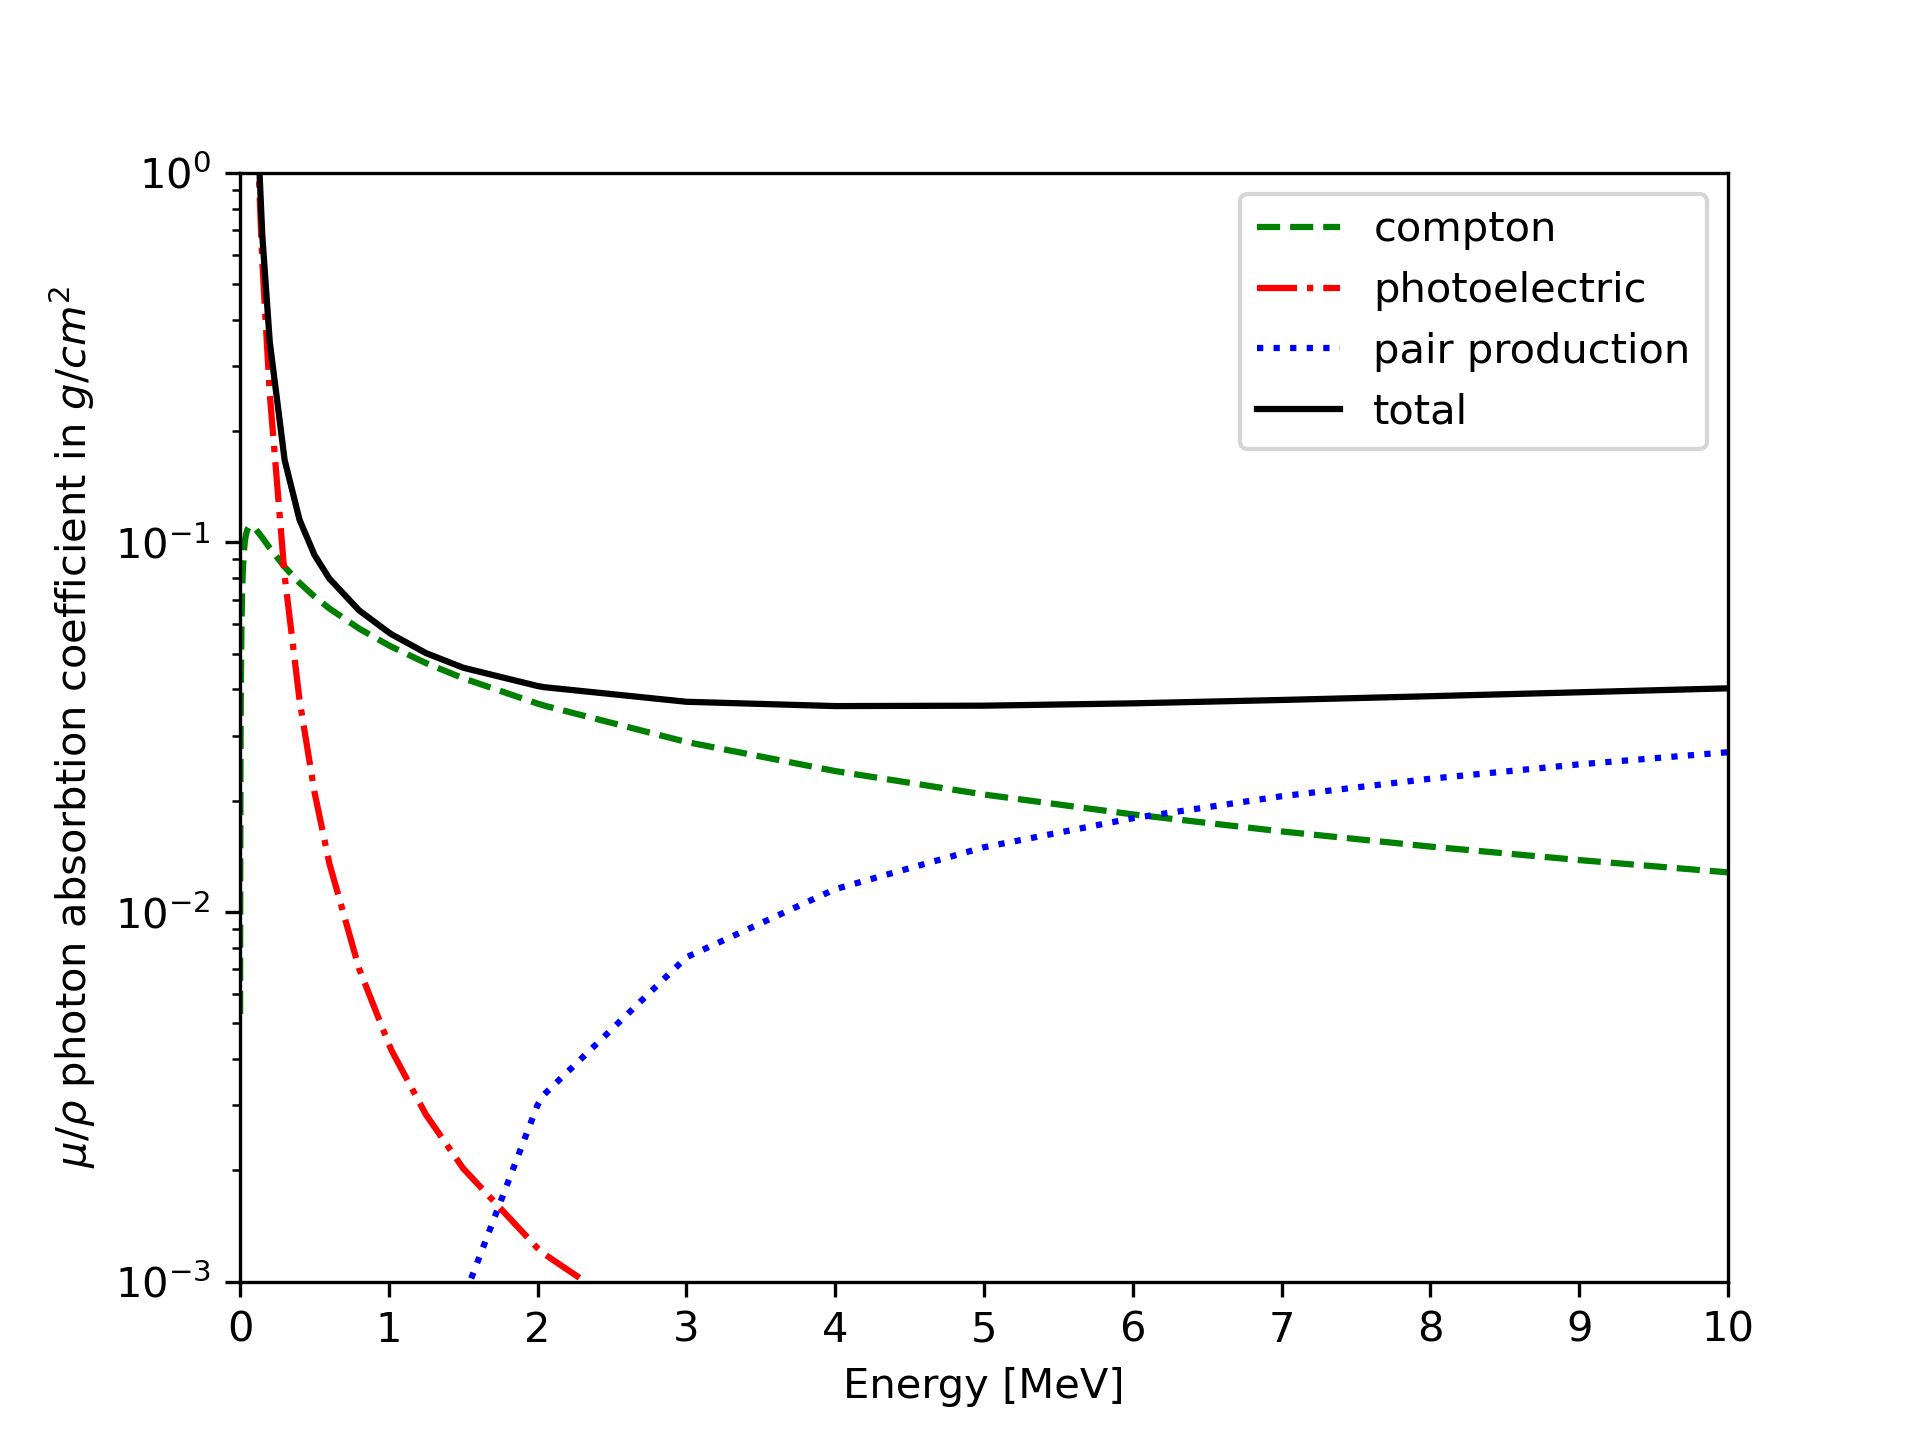
\includegraphics[width=0.49\textwidth]{csi_attuenuation.png}	
	\caption{Mass attenuation coefficients for photons in CsI in the range from $100$ keV to $20$ MeV according to XCOM database\cite{seltzer2010xcom}.} 
	\label{fig:csi}%
\end{figure}
At photon energies below approximately $300$ keV, the photoelectric effect dominates the interaction cross-section. As the photon energy increases, Compton scattering becomes the predominant process. For photon energies exceeding the pair production threshold ($E_{\gamma} > 2m_{e}c^2 \approx 1.022 MeV$), electron-positron pair creation becomes possible and is the dominant interaction mechanism above $\backsim 6$ MeV.\newline
Compton scattering broadens the clustering by the deflection of the incident gamma ray. According to the Klein–Nishina formula, the scattering is predominantly forward-focused for moderate to high photon energies\cite{klein1929streuung}, leading to clusters in neighboring crystals.\newline
In the case of pair production, which occurs above the $2m_ec^2$ threshold, the resulting annihilation of the positron yields two $511$ keV gamma photons. These secondary photons often escape the initial interaction site, leading to a significant fraction of the incident photon’s energy being deposited in multiple detector elements.\newline
For gamma rays emitted by nuclei at rest, this behavior gives rise to well-defined single- and double-escape peaks in the recorded energy spectra -- corresponding to the escape of one or both $511\,\mathrm{keV}$ photons, respectively -- if these photons exit the cluster volume without interaction (see Fig. X).\newline
In experiments involving relativistic ions, such as those conducted at $R^3B$, Doppler broadening significantly distorts spectral features, including single- and double-escape peaks. This effect hinders accurate reconstruction of the photon energy and complicates the extraction of absolute gamma-ray yields and reaction cross sections.

\subsection{Data Structure and Standard R3B Clustering Algorithm}\label{s_sec:r3b_clustering}
In the standard data acquisition (DAQ) configuration, all CALIFA detector hits occurring within a $\pm 4\,\mu\mathrm{s}$ time window are grouped into a single event. Each individual hit $i$ in CALIFA is represented by a data structure containing the following calibrated information:
\begin{itemize}
    \item Energy deposit $E_i$
    \item Polar angle $\theta_i$
    \item Azimuthal angle $\phi_i$
    \item Time stamp $t_i$ (via White Rabbit  Precision Time Protocol\cite{lipinski2011white})
\end{itemize}
In the standard R3B clustering approach, the time information $t_i$ is not utilized during the spatial reconstruction of clusters.\newline
The initial stage of the clustering algorithm begins by sorting all hits in descending order of energy. A user-defined geometric condition, typically a conical cluster shape with a default aperture of $0.5\,\mathrm{rad}$, is applied. This value has been found to provide an optimal compromise between compact high-energy clusters and more diffuse gamma-ray showers.\newline
The hit with the highest energy defines the seed or center of the first cluster. The algorithm then iterates through the remaining hits and includes each hit in the current cluster if it lies within the specified cone aperture relative to the seed direction. Once the list is fully processed for the current cluster, the next highest-energy unassigned hit becomes the seed of a new cluster. This procedure repeats until no unassigned hits remain.\newline
\subsection{Simulation Setup}\label{s_sec:data_sim}
To evaluate and compare the clustering algorithms presented in this work, simulated data are required, as supervised machine learning approaches rely on access to ground truth labels. For this purpose, the R3BROOT framework with a Geant4-based Monte Carlo \cite{agostinelli2003geant4} backend was employed.\newline
The CALIFA detector geometry used in the simulation corresponds to the configuration implemented in early 2024. At that time, the iPhos region (polar angles $19^\circ$ -- $43^\circ$) was fully instrumented, while only the forward half of the Barrel region ($43^\circ$ -- $87^\circ$) was active. The forward-most CEPA region ($7^\circ$ -- $19^\circ$) was not yet equipped.\newline
Gamma-ray energies were sampled from a uniform distribution between $0.3\,\mathrm{MeV}$ and $10\,\mathrm{MeV}$. The interaction of the primary gamma rays with the CsI(Tl) scintillation material was modeled using Geant4 transport physics.\newline
To emulate realistic event topologies, three gamma rays were generated per event, resulting in multiple detector hits. Timing information was coarsely simulated by assigning each primary gamma a random emission time within the $\pm 4\,\mu\mathrm{s}$ event window. The corresponding hit times were then Gaussian-smeared with a standard deviation of $200\,\mathrm{ns}$ to reflect typical electronic channel timing variations.\newline
The resulting dataset was split into training and test subsets, comprising 13{,}000 and 7{,}000 events, respectively.


\subsection{Preformance Metrics}\label{s_sec:metrics}
To quantitatively assess the performance of the clustering algorithms presented in this work, a set of four custom metrics was defined. Three of these are event-based, while an optional fourth metric evaluates clustering quality on a per-cluster basis:
\begin{itemize}
    \item \textbf{True Positive (TP)}: All hits in an event are correctly assigned to their respective clusters.
    \item \textbf{False Positive (FP)}: At least one hit in an event is incorrectly merged into a cluster it does not belong to.
    \item \textbf{False Negative (FN)}: At least one hit is not merged into its true cluster and instead forms a spurious cluster.
    \item \textbf{False Mixed (FM)}: An event is classified as false mixed if it contains both FP and FN characteristics—i.e., at least one hit is wrongly assigned, and at least one true cluster is partially reconstructed.
\end{itemize}
In addition, a cluster-based metric is defined:
\begin{itemize}
    \item \textbf{Well Reconstructed (WR)}: The ratio of correctly reconstructed clusters to the total number of true clusters in the dataset.
\end{itemize}
These metrics allow a comprehensive evaluation of clustering accuracy, robustness, and failure modes.

\subsection{Agglomerative Clustering}\label{s_sec:agglo}
To incorporate temporal information into the clustering process---unlike the standard R3B algorithm, which omits it---a generic, well-established method was adopted: agglomerative clustering as implemented in the \texttt{fclusterdata} function from the \texttt{SciPy} library. This approach enables flat clustering based on hierarchical linkage with a user-defined threshold.\newline
Each hit was mapped into spherical coordinates \((\theta, \phi, r)\), where the radial component \(r\) encodes time information. To ensure non-negative radii, the acquisition time window of \(\pm 4\,\mu\mathrm{s}\) was shifted by \(+4.5\,\mu\mathrm{s}\). The Ward linkage criterion \cite{nielsen2016hierarchical}, which minimizes intra-cluster variance, was employed as the distance metric.\newline
The threshold parameter was optimized to yield the best performance according to the custom-defined metrics. A comparison between the standard R3B clustering and the agglomerative method is presented in Fig.\ref{fig:r3b_agglo_metrics}.
\begin{figure}[!htb]
	\centering 
	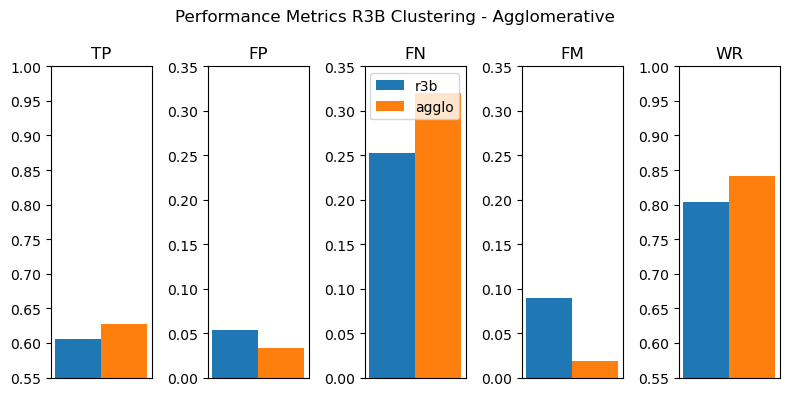
\includegraphics[width=0.4\textwidth]{r3b_vs_agglo_metrics.png}	
	\caption{Comparison of clustering performance on the test dataset using standard R3B clustering (blue) and agglomerative clustering (orange) incorporating hit-time information. The dataset comprises simulated $\gamma$-rays with energies uniformly distributed between 0.3 and 10\,MeV. The metrics shown include event-based and cluster-based measures: \textit{well\_reco}, \textit{true\_positive}, \textit{false\_positive}, \textit{false\_negative}, and \textit{false\_mixed}.} 
	\label{fig:r3b_agglo_metrics}%
\end{figure}
As shown in Fig. \ref{fig:r3b_agglo_metrics}, the agglomerative clustering algorithm demonstrates improved performance both on an event level (true positive rate) and on a cluster level (correctly reconstructed clusters). However, this improvement is accompanied by an increased false negative rate, indicating that the algorithm tends to under-merge hits near the edges of clusters. This limitation motivated the development and application of an edge detection neural network, which is introduced in the following subsection.


\subsection{Implementation of the Edge Detection Neural Network}\label{s_sec:edge}
To enhance the clustering performance, particularly at the boundaries of hit distributions, a generic neural network (NN) was developed to perform pairwise classification of detector hits. This model is applied either to individual raw hits or to hits pre-clustered via agglomerative clustering, on an event-by-event basis.

The model takes 12 input features for each hit pair $(i, j)$: absolute values of energy $(E_i, E_j)$, polar angle $(\theta_i, \theta_j)$, azimuthal angle $(\phi_i, \phi_j)$, and time $(t_i, t_j)$. Additionally, four differential features are computed: $\Delta E = |E_i - E_j|$, $\Delta \theta = |\theta_i - \theta_j|$, $\Delta \phi = |\phi_i - \phi_j|$, and $\Delta t = |t_i - t_j|$. These differential inputs are essential for training stability and convergence. In particular, $\Delta \phi$ resolves the discontinuities caused by the periodicity of the azimuthal angle (e.g., distinguishing between $\phi = 355^\circ$ and $\phi = 5^\circ$), which would otherwise introduce large erroneous differences in angular comparisons.

Of the 12 features, only the hit time is normalized to the $[0, 1]$ interval; all other values are used in their native physical units.

The architecture of the neural network is illustrated in Fig. \ref{fig:architecture}. The 12-dimensional input vector is passed through a fully connected feed-forward network with one hidden layer of $10^3$ nodes, followed by a ReLU activation. Two additional hidden layers, each with $10^2$ nodes, are applied sequentially. The output layer consists of a single node with a sigmoid activation, yielding a score in the interval $[0, 1]$, where values close to 1 indicate that the hits (or clusters) are likely to originate from the same event cluster.
\begin{figure}[!htb]
	\centering 
	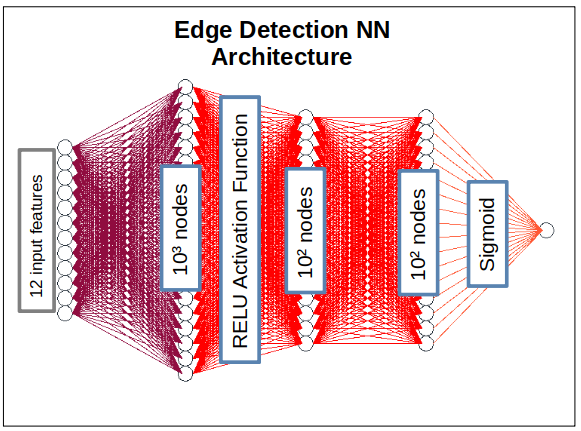
\includegraphics[width=0.4\textwidth]{architecture.png}	
	\caption{Schematic architecture of the edge detection neural network. The model consists of three fully connected hidden layers. The final output layer comprises a single node with a sigmoid activation function, yielding a prediction score in the range $[0, 1]$. Values closer to 1 indicate that the input hit pair originates from the same physical cluster and should be merged, while values near 0 suggest they should remain separate.}
	\label{fig:architecture}%
\end{figure}

Training is performed using the binary cross-entropy loss function\cite{mannor2005cross}\cite{de2005tutorial} and stochastic gradient descent (SGD)\cite{newton2018recent} with a fixed learning rate of $5 \times 10^{-3}$. Given the moderate size of the training dataset, full-batch training is employed without mini-batching. The model is trained for $8 \times 10^5$ epochs. After training, a tunable threshold is applied to the prediction scores to classify hit pairs. Final clusters are then formed by grouping all connected hit pairs based on the predicted associations.

The edge detection NN was implemented and tested in three configurations:

\begin{itemize}
    \item \textbf{Plain Edge NN:} The model is applied directly to individual hits without any pre-clustering. All clustering is performed based solely on the NN predictions.

    \item \textbf{Agglomerative + Edge NN:} The data is first clustered using the agglomerative algorithm described in the previous subsection. For each resulting cluster, an energy-weighted center of mass is calculated, replacing individual hits. The NN is then trained on false negative cases (i.e., under-merged hits) from this initial clustering. In application, agglomerative clustering is first applied to the test data, followed by the NN to refine the boundaries and reduce the false negative rate (see Fig.\,2).

    \item \textbf{R3B Clustering + Edge NN:} This configuration mirrors the Agglomerative + Edge NN approach, but omits the use of time information. In line with the standard R3B clustering methodology, the time inputs are fixed to a constant value of 1 to reflect their exclusion from the clustering process.
\end{itemize}

%To support agglomerative clustering in identifying edge hits, a generic neural network architecture was developed to perform pairwise comparisons of individual hits. This was applied either directly to the raw hit data or to pre-clustered hits obtained via the agglomerative clustering algorithm on an event-by-event basis.
%
%The model processes 12 input features, describing a pair of hits \(i\) and \(j\): the absolute values of energy \(E_i, E_j\), polar angles \(\theta_i, \theta_j\), azimuthal angles \(\phi_i, \phi_j\), and times \(t_i, t_j\). In addition, four differential features are computed: \(\Delta E = E_i - E_j\), \(\Delta \theta = \theta_i - \theta_j\), \(\Delta \phi = \phi_i - \phi_j\), and \(\Delta t = t_i - t_j\). These differential features are essential for model convergence, especially \(\Delta \phi\), which accounts for the periodic nature of azimuthal angles and mitigates discontinuities (e.g., between \(355^\circ\) and \(5^\circ\)). Without these, the model encounters convergence issues due to misleading distance estimates in angular space.
%
%Among the input features, only the hit time is normalized to the [0, 1] range; energy and angular values are used in their raw form.
%
%The architecture of the edge detection neural network is shown in Fig.\,X. The 12 input features are processed by a fully connected feedforward network. The first hidden layer consists of \(10^3\) nodes with ReLU activation, followed by two additional hidden layers of \(10^2\) nodes each. A final sigmoid activation is applied to a single-node output layer, yielding a probability score between 0 and 1. A value close to 1 indicates that the two hits (or clusters) belong to the same cluster; a value near 0 indicates otherwise.
%
%Model training uses the binary cross-entropy loss function and stochastic gradient descent optimization with a fixed learning rate of \(5 \times 10^{-3}\). Due to the manageable dataset size, full-batch training is performed without the need for mini-batching. The model is trained for \(8 \times 10^5\) epochs. Final classification is performed by applying a tunable prediction threshold to optimize the clustering performance on the validation dataset.
%
%The edge detection neural network is applied in three configurations:
%
%\begin{itemize}
%    \item \textbf{Plain Edge NN:} The model is used as a standalone clustering tool based solely on pairwise hit comparisons, without any prior agglomerative clustering.
%    
%    \item \textbf{Agglomerative + Edge NN:} The dataset is first pre-clustered using the agglomerative algorithm described in the previous subsection. For each cluster, an energy-weighted center-of-mass is calculated, replacing the individual hits. The edge detection model is trained on false negative cases from the agglomerative clustering step. During inference, the model is applied to the pre-clustered data to improve merging at the cluster boundaries, particularly reducing the false negative rate (see Fig.\,2).
%    
%    \item \textbf{R3B Clustering + Edge NN:} Similar to the previous configuration, but consistent with the standard R3B clustering approach, the hit time information is omitted by assigning a constant value of 1 to the corresponding input features.
%\end{itemize}
%\begin{figure}
%	\centering 
%	\includegraphics[width=0.4\textwidth, angle=-90]{JHEAP_cover_image.pdf}	
%	\caption{High Energy Astrophysics journal cover} 
%	\label{fig_mom0}%
%\end{figure}

%A random equation, the Toomre stability criterion:
%
%\begin{equation}
%    Q = \frac{\sigma_v \times \kappa}{\pi \times G \times \Sigma}
%\end{equation}

\section{Results}\label{sec:results}
\begin{table}[h!]
\begin{center}
\begin{tabular}{||c| c| c |c | c|| c|}
 \hline
 Clustering Model & TP & FP & FN & FM & WR \\ [0.5ex] 
 \hline\hline
 R3B Standard Clustering & 60.6 & 5.3 & 25.2 & 8.9 & 80.4 \\ 
 \hline
 Agglomerative Clustering & 62.8 & 3.3 & 32.0 & 1.9 & 84.1 \\ 
 \hline
 Edge Clustering (no time) & 63.4 & 7.2 & 24.8 & 4.6 & 82.4 \\ 
 \hline
 Edge Clustering (with time) & 74.7 & 3.4 & 20.5 & 1.4 & 89.2 \\ 
 \hline
 R3B + Edge (no time) & 67.4 & 8.5 & 16.0 & 8.0 & 82.2 \\ 
 \hline
 Agglo + Edge (with time) & 81.3 & 5.1 & 12.2 & 1.5 & 91.0 \\
 \hline
\end{tabular}
\end{center}
%\caption{Overview of the resulting performance metrics, as introduced in subsection \ref{s_sec:metrics}, for the various clustering models.The models \textit{R3B Standard Clustering},\textit{Edge Clustering (no time)},\textit{R3B + Edge (no time)} use the angular and energy hitwise information, the models \textit{Agglomerative Clustering},\textit{Edge Clustering (with time)} and \textit{Agglo + Edge (with time)} use in addition also the hit-time for cluster reconstruction.}
\caption{Summary of performance metrics as defined in Subsection~\ref{s_sec:metrics}, evaluated for the different clustering algorithms. The models \textit{R3B Standard Clustering}, \textit{Edge Clustering (no time)}, and \textit{R3B + Edge (no time)} utilize angular and energy information on a per-hit basis for cluster reconstruction. In contrast, \textit{Agglomerative Clustering}, \textit{Edge Clustering (with time)}, and \textit{Agglo + Edge (with time)} additionally incorporate time-of-hit information into the clustering process.}
\label{tab:results}
\end{table}
The results of this study are summarized in Table~\ref{tab:results}, where the ordering of the clustering models reflects the methodological workflow followed during the investigation. The initial comparison was conducted between the baseline \textit{R3B Standard Clustering} algorithm and a generic \textit{Agglomerative Clustering} model that incorporates time-of-hit information.\newline
The agglomerative model shows improved performance over the R3B baseline in terms of both event-level true positives (TP) and cluster-level (WR) values. However, it exhibits inferior performance with respect to the false negative (FN) rate, indicating a tendency to miss relevant hits during reconstruction. This limitation motivated the development of an Edge Detection Neural Network, initially evaluated as a standalone clustering algorithm and subsequently integrated into the agglomerative framework, yielding the combined model denoted as \textit{Agglo + Edge}.\newline
The \textit{Agglo + Edge} model demonstrates superior performance across all evaluated metrics, achieving an overall correct reconstruction rate of 81.3\%, significantly outperforming the \textit{R3B Standard Clustering} algorithm, which reaches 60.6\%.\newline
To further explore the capabilities of neural network-based clustering approaches, two additional models were evaluated: a standalone \textit{Edge Detection Neural Network} and a hybrid approach combining \textit{R3B Standard Clustering} with edge-based postprocessing (\textit{R3B + Edge}). Notably, both of these models operate without incorporating time-of-hit information, similar to the R3B baseline. Nonetheless, both outperform the \textit{R3B Standard Clustering} in all reported metrics, underscoring the potential of edge-based neural network models for improving cluster reconstruction in high-granularity detector systems.


%r3b,0,0.804,0.606,0.053,0.252,0.089
%agglo,0,0.841,0.628,0.033,0.320,0.019
%edge_no_time,0,0.824,0.634,0.072,0.248,0.046
%edge_with_time,0,0.892,0.747,0.034,0.205,0.014
%agglo_edge,0,0.910,0.813,0.051,0.122,0.015
%r3b_edge,0,0.822,0.674,0.085,0.160,0.080


%\begin{table}
%\begin{tabular}{l c c c} 
% \hline
% Source & RA (J2000) & DEC (J2000) & $V_{\rm sys}$ \\ 
%        & [h,m,s]    & [o,','']    & \kms          \\
% \hline
% NGC\,253 & 	00:47:33.120 & -25:17:17.59 & $235 \pm 1$ \\ 
% M\,82 & 09:55:52.725, & +69:40:45.78 & $269 \pm 2$ 	 \\ 
% \hline
%\end{tabular}
%\caption{Random table with galaxies coordinates and velocities, Number the tables consecutively in
%accordance with their appearance in the text and place any table notes below the table body. Please avoid using vertical rules and shading in table cells.
%}
%\label{Table1}
%\end{table}


\section{Discussion and Outlook}\label{sec:disc_outlook}

The results presented in the previous section clearly demonstrate that high-level machine learning approaches, such as the Edge Detection NN, can significantly enhance the accuracy of cluster reconstruction. These models not only reduce distortions in the measurement process but also exhibit increased sensitivity to low-statistics reactions—an important feature for experiments targeting rare processes.\newline
It is noteworthy that even the models, which do not utilize time-of-hit information (similarly to the \textit{R3B Standard Clustering}), outperform the baseline method. This underscores the general effectiveness of neural network-based methods in extracting structural features from detector data.\newline
The inclusion of time-of-hit information proves to be a critical factor for enhancing clustering performance. As this observable is typically available for CALIFA at R$^3$B, the results of this study support the recommendation to incorporate it into the reconstruction pipeline wherever possible.\newline
Furthermore, these findings are intended to encourage broader adoption of advanced machine learning techniques by experimental groups, particularly in setups involving highly granular detectors. Such tools offer substantial performance benefits and can support more precise event reconstruction.\newline
However, a consideration of computational complexity is essential. Both the \textit{R3B Standard Clustering} and \textit{Agglomerative Clustering} methods exhibit a time complexity of $\mathcal{O}(N^2)$\cite{sieranoja2025fast}, where $N$ is the number of hits. The proposed \textit{Edge Detection Neural Network}, whether used in standalone mode or as an auxiliary module (\textit{R3B + Edge}, \textit{Agglo + Edge}), requires additional computational resources. In particular, the neural network involves large matrix operations—for instance, the second fully connected layer with $10^3$ input and $10^2$ output features—whose computational cost dominates for events with $N \sim \mathcal{O}(10^1)$. Consequently, the current implementation is not suitable for online processing and is better suited for detailed offline analyses, where accuracy is prioritized over execution speed.\newline
Future work should focus on optimizing the Edge Detection Neural Network for speed and scalability. Additionally, transformer-based models\cite{vaswani2017attention}—capable of analyzing full event topologies—may offer further improvements in clustering accuracy by capturing complex, global features.

\section*{Acknowledgements}
The work was supported by BMBF 05P24WO2 and Excellence Cluster ORIGINS from the DFG (Excellence Strategy EXC-2094-390783311).

%% The Appendices part is started with the command \appendix;
%% appendix sections are then done as normal sections
\appendix

\section{Appendix title 1}
%% \label{}

\section{Appendix title 2}
%% \label{}

%% If you have bibdatabase file and want bibtex to generate the
%% bibitems, please use
%%
\bibliographystyle{elsarticle-num} 
\bibliography{literature.bib}

%% else use the following coding to input the bibitems directly in the
%% TeX file.

%%\begin{thebibliography}{00}

%% \bibitem[Author(year)]{label}
%% For example:

%% \bibitem[Aladro et al.(2015)]{Aladro15} Aladro, R., Martín, S., Riquelme, D., et al. 2015, \aas, 579, A101


%%\end{thebibliography}

\end{document}

\endinput
%%
%% End of file `elsarticle-template-harv.tex'.
